\newpage\thispagestyle{empty}\newpage\chapter[Mathematica \protect\~{} 一切都是表达式]{Mathematica \~{} 一切都是表达式}\label{cp:Mathematica}
\addauthor{小飞舞}
\medskip
\begin{tcolorbox}[colback=gray!15!white,
        colframe=black!80,
        arc=1mm, auto outer arc,
        boxrule = 0.5pt,
        title=前言,breakable,
        fontupper = \itshapeCJK
    ]
    幻想乡内白雪皑皑,漫山遍野披上了银装:一眨眼,冬天又到了,人类、妖精们都穿上了胖乎乎的冬装准备迎接年末的宴会。\bigskip

    可能是这博丽巫女最近看外界的奇怪书看上头了,这次宴会她决定在畅饮之前弄个“文化交流宣传”的什么东西。届时,妖怪、人类、妖精们都会来博丽神社鸟居前摆摊,按照这博丽巫女的说法:

    “这将极大地促进人类与妖怪之间的有效交流,同时也可以让幻想乡的文化多样性焕发出勃勃生机。”

    虽然是官腔官调,但这的确能在人类村落里引起相当的轰动——往年的“摆摊”只是售卖零食、小吃一类的消遣玩意,现在又多了个“文化交流”的噱头出来,那确实能够吸人眼球。\bigskip

    想要在人类村落争取一把影响力的天狗、河童等群体也跃跃欲试。既然巫女已经网开一面,自己再不争取也只是纯粹的丢把子——当然,高层对这破事肯定是不重视的,这破村落的摊,能值几个钱?还不如去外面卖同人本本。反正最后放开了也是加剧那群不懂事的信息内战,最后搞得草草收场留不下什么印子。\bigskip

    尽情玩吧!反正最后大家都谈拢了,人类也好,妖怪也罢,反正就当做过个新年吧。山上的那几个老家伙就这么传令下去。这命令本源自那红白,现在借由这妖怪山最大的广告势力沿着全幻想乡铺展开。\bigskip

    这知情者一多了就开始麻烦——博丽神社就是个穷苦地方,开点小摊还好,这那么多人马一来这里就显得非常尴尬。这博丽就在那一直摊手,这一摊就摊了个分会场出来:把天狗和河童那些玩意都丢到魔法森林分会场去!让森林里那些老家伙会会如今的幻想乡自媒体新生代。\bigskip

    我们这故事就发生在那片魔法森林里。
\end{tcolorbox}

\setcounter{section}{0}
\setlength{\parindent}{2em}

\section{首要的例子}


\begin{center}
    \begin{tcolorbox}[colback=gray!15!white,%gray background
            colframe=black!80,% black frame colour
            arc=1mm, auto outer arc,
            boxrule=0.5pt,
            title=序,
            fontupper = \itshapeCJK
        ]森林里好不热闹——来访的家伙们大多不是人类,有各种各样的妖怪、也有跑来凑热闹的小妖精,甚至连那高高在上的大天狗本人也偷偷来这尘世视察一下。\bigskip

        些许是被赶出中心区的原因,妖怪山那俩种族就在那边喝酒边扯皮边卖些没有营养的东西。不过好在还管得住嘴,气氛勉强能够缓慢推进。\bigskip

        “哟!这不是老霖吗!”发言的正是九尾天狐八云蓝,穿着一条简洁的白色长裙,领口绣着小花,她依然用帽子遮着自己耳朵,与此对比鲜明的是九条硕大的尾巴张扬地跟在后面。森林这地可不像博丽神社那样有规矩,大家早早就把酒满上了,现在即使是她也有些微醉。\bigskip

        “原来是蓝小姐啊……”,作为摊主的森近霖之助满脸堆笑,沽溜地想了会,没啥可说的,“真想不到您也会来。”\bigskip

        就这样寒暄道。\bigskip

        “嘛……就没事来看看,听说这里还有油豆腐卖?”月光撒在大妖怪身上,如同幻梦一般魅惑。\bigskip

        那店主想了想,“撒……这油豆腐嘛……估摸着在神社那附近吧,这里只有些没用的新闻。”附近那么多天狗,他也不好说什么坏话。见八云蓝没有回应——\bigskip

        “看看这个?”霖之助决定上自己的杀手锏,他稍稍侧开身位,让月光能够慢慢弥漫到他身后的女孩附近。那女孩身着精致的黑色连衣裙,不过看起来相当保守——毕竟是冬天的缘故,背后一支褐色的翅膀耷拉在地上,另一支索性搭在她面前桌子上的一个巨大平板上面。不知道在对着书鼓捣着什么。\bigskip

        “这个是我偷偷从外界收来的——新型的电脑!比那之前的老古董好多了。”森近自豪地介绍道。那女孩的翅膀也因此随之动颤——猛然间收紧,带起一大片泥土,差点把那黑不溜秋的大平板打翻在地。\bigskip

        “霖之助霖之助,那位是谁哇?”她就用这么不大不小的声音问道,倒是八云蓝本人作出了回答:“在下是妖怪八云蓝,请多多指教。”\bigskip

        “是之前算出三途河宽度的数学大师八云蓝小姐吗?久仰久仰。”无名的读书妖怪也报以礼貌性的寒暄。在那霖之助的介绍下,这八云蓝也被那“电脑”勾起了兴趣。\bigskip

        “这种东西看起来的确是从外界来的——在这里居然可以正常使用。”八云蓝微微惊叹道,对着平板——所谓的液晶显示器上面的图像露出姨母笑,“这玩意可以用来干嘛?看样子好像有个可交互的那什么来着……”\bigskip

        “桌面吧,”那女孩说,“蓝小姐可能对这个感兴趣……”隔着臃肿的手套,无名妖怪在一片破旧的机械键盘上面按着方向键。古老的机械键盘会随着桌子微微颤动,当少女轻触键盖时就会发出幽怨的咯哒声——“这键盘可能还比那巫女年长咧”。霖之助这么说道,“多亏这位女孩这电脑才可以连上这……呃,输入设备。”
    \end{tcolorbox}
\end{center}

“打开了。”少女平静的声音传过来。

\begin{center}
    \bigskip
    
\includegraphics[width = 0.3\textwidth]{Mathematica.pdf}

    \begin{tcolorbox}[skin = enhanced,
            interior style = {left color = white, right color = white, middle color = EE6743!80!red}, width = .5\textwidth, boxrule = 0pt, colframe = white, boxsep = 0pt, top = 2pt, bottom = 1pt, sharp corners,
        ]
        \footnotesize\sffamily\centering\color{white} Initializing kernels\dots
    \end{tcolorbox}
\end{center}

“草,好丑的配色。”八云蓝笑嘻嘻地揶揄道。

很快,那奇怪的标志消失了,在等待了许久之后,弹出了一个几乎是纯白色的窗口:

\begin{notebook}{Untitled-1 * - Wolfram Mathematica 13.1}
    \rule[1em]{1em}{1pt}\mbox{}\vspace*{10em}
\end{notebook}

“这是什么?”八云蓝虽然这样问了,但从这界面大概也猜得出个大概:这玩意估摸着是打代码的——最顶上的光标一闪一闪,仿佛在等待着什么。

“这是一个CAS\footnote{Computer Algebra System, 计算机代数系统。},几乎是人类现代数学技术计算的结晶之一。”这鸟妖怪边看那屏幕边说。

“数学计算?”那名不虚传的数学大师终于将脸蹭过来,仿佛古神低语的声音刺破嘈杂的空气,但缓慢悠长地传到那朱鹮的耳朵里。“有趣”,她最后用孤山妖怪般令人脊背发凉的声音这么说道。

“这样吧,让我看看这玩意能干嘛,”最后,八云大师这样说道,她抛出了一个简单的不定积分:$\int \frac{1}{t^4-1} \, \mathrm{d}t .$

\begin{notebook}{Untitled-1 * - Wolfram Mathematica 13.1}
    \def\textit#1{{\color{cyan!60!black}#1}}
    \mmain\texttt{ Integrate[1 / (\textit{t}\char"005E 4 - 1), \textit{t}]}
    \tcblower
    \mmaout\[
        \frac{1}{4} \log (1-t)-\frac{1}{4} \log (t+1)-\frac{1}{2} \tan ^{-1}(t)
    \]
\end{notebook}

“还行”,八云蓝应付道,这样容易的积分的确没啥意思,就在她的目光在那屏幕上肆意游走时,她看到了这窗口的标题栏:

\begin{center}
    \sffamily Wolfram Mathematica
\end{center}

这 Mathematica 的名字有点意思……她自然而然地这么想,至于那前面的 Wolfram……估摸着是人名吧。

“这玩意挺有意思的,”见九尾狐没有再发问,那鸟妖怪的眉心也慢慢舒展——如同被技艺高超的按摩大师抚平一般,“试试看?”最后抛出了一句带有期待性的试探。

这平凡的试探自然逃不过八云的察觉,她清楚那无名妖怪想要和自己介绍那玩意——被称为“人类现代数学技术计算的结晶之一”的神奇玩意。作为幻想乡最有分量的式神,自然对被称为“外界式神”的电脑有所耳闻,不过此时面临的是自己毫无把握的“技术结晶”,自己必然有义务好好了解者个稀奇古怪的玩意。

“你先介绍下这玩意吧,我还不知道这是什么。”爱屋及乌地,八云蓝对数学地兴趣自然而然的转移到这红白软件上来。

“啊……我自己也不是很——哦有了”,那鸟妖怪在任务栏搜寻着:\texttt{Help > Wolfram Website},然后瞬间地——有另外一个窗口弹了出来,在顶上的食尾蛇旋转了几十圈之后,才勉强地打开了一个网站:

\url{https://www.wolfram.com/}

\newtcolorbox{website}[1]{
    enhanced,
    clip upper = true,
    left = -3pt,
    top = -3pt,
    right = -3pt,
    bottom = -3pt,
    colframe = lightgray!40!white,
    title = {\
            \begin{tikzpicture}
                \filldraw[macred] (0, 0) circle (0.3em);
                \filldraw[macyellow!80!white] (0.5, 0) circle (0.3em);
                \filldraw[macgreen] (1, 0) circle (0.3em);
            \end{tikzpicture}%
            \hfill{\footnotesize\sffamily #1}\hfill%
            \phantom{
                \begin{tikzpicture}
                    \filldraw[macred] (0, 0) circle (0.3em);
                    \filldraw[macyellow!80!white] (0.5, 0) circle (0.3em);
                    \filldraw[macgreen] (1, 0) circle (0.3em);
                \end{tikzpicture}
            }
        }, coltitle = black, sidebyside, righthand ratio = 0.02, colbacklower = red!20, sidebyside gap = 0mm, sidebyside align = top seam, height = 0.5\paperheight}

\begin{website}{{https://www.wolfram.com}}
    \makebox[\width][c]{
\includegraphics[width = \linewidth]{Wolfram.pdf}}

    \vspace*{-10em}
    \tcblower
    \smallskip
    \centerline{\begin{tikzpicture}[scale = 0.05]
            \filldraw[gray] (0, 0) -- (0.5, 0) -- ++ (1, 1) --++ (1, -1) -- ++ (0.5, 0) --++ (-1.5, 1.5) -- cycle;
        \end{tikzpicture}}
    \smallskip

    \color{gray}\rule{1em}{12em}
\end{website}

全面的……计算语言?那确实挺大胆的。策士心中这样认为,但更让她恼火的事情反而是这个硕大的,十分嚣张出现在屏幕上面的狐狸 Logo\footnote{估摸着这更可能是狼 (Wolf),但是我不听我不听我不听我不听我不听我不听我不听我不听我不听我不听我不听我不听我不听我不听我不听我不听我不听我不听我不听我不听我不听我不听我不听我不听我不听我不听——},看起来就像在调挑衅自己一般。看来人类的科技发展到了一个相当令人敬畏的地步啊……在自己还没来到幻想乡的年代,他们还什么都不是呢。她想,这样一来,既然眼前这鸟妖怪能够如此熟练地使用人类开发出来的这些乱糟糟的玩意,想必也是“人类化”相当严重的妖怪吧。

“有趣,人类为了求解数学问题居然开发了这样的‘式’”,狐妖评论道,“那让我看看这玩意到底有多大能耐吧。”

朱鹭子警惕地望着她。



\section{八云蓝与 Mathematica}



\begin{center}
    \begin{tcolorbox}[colback=gray!15!white,
            colframe=black!70,
            arc=1mm, auto outer arc,
            boxrule=0.5pt,
            title=序,
            fontupper = \itshapeCJK
        ]
        这八云蓝倒也爽快——只要这“式”,或者说软件能够回答出八云蓝出的题目就可以,事实上,那鸟妖怪也想趁这个机会来宣传一下什么人类科技的结晶——在河童天狗中间。两位妖怪当下就达成了意见一致:就请这位和天狗女郎们喝得醉醺醺的老霖当什么“见证人”之类,然后就拉一摞子天狗河童过来宣传。\bigskip

        天狗们倒全都是喝不醉的好事之徒,这整个社会结构的技术力量来源都要靠河童的帮助,而河童又要靠那用自己“有远见的神威”压在桌子上碾着对方谈判的神奈子来引入外界的新潮技术。总之就是——大家都希望这长得像那博丽巫女的新潮玩意可以机械降神,一股脑保证这两个种群的发展,而不是求请于山顶上的那位自诩神明的资本家。\bigskip

        都来了兴致,就这么有些人就围过来了,大家都想看看这比赛……哦不,是新产品的发布会到底有什么乐子。\bigskip

        “不!禁止记录!”察觉到由所谓“记者灵魂”驱使着的天狗的接近,八云蓝大声说道,她站起来,最强式神的称号加上她那不怒自威的神色,令所有天狗都不敢再靠前:这家伙背后可是有一个强得没边的管理者存在,即使天狗们打得过这位妖狐,恐怕也要遭受武力和舆论两大威胁。\bigskip

        在没收了天狗们所有的笔和相机之后,八云蓝总算同意开始了。
    \end{tcolorbox}
\end{center}

\subsection{第一乐章:轻快的小快板}

“比赛”初期的气氛是非常活泼的——八云蓝也并不想为难这软件:即使是自己也有很多算不出来的东西,但身为“式”,最擅长的并不是在一个领域的登峰造极,而是如同大海一般将所有领域都包围与其中。就先从简单开始吧,八云蓝这样想:

先试试解方程吧,她说。

\[
    x^3 + 4x -  4 = 0
    .\]
河童们当然是能看懂这玩意的,天狗也有不少可以——最惨的估计是老霖,这符号他肯定在某些书上见过,也知道可以用来干嘛,但是具体怎么用他的确是一窍不通。

那无名妖怪在那软件里面输入 \verb"Solve[x^3 + 4x - 4 == 0, x]",然后按了 \verb"Shift + Enter"——

\begin{mathematica}
    Solve[\key{x}\^3 + 4x - 4 == 0, \key{x}]
    \ShiftEnter
    \{\{x -> Root[-4 + 4*\#1 + \#1\^3 \&, 1]\},

    \{x -> Root[-4 + 4*\#1 + \#1\^3 \&, 2]\},

    \{x -> Root[-4 + 4*\#1 + \#1\^3 \&, 3]\}\}\footnote{这里返回奇怪代码的原因为了方便输入,事实上在 Mathematica 中 \EscVerb{x -> Root[-4 + 4*\#1 + \#1\^3 \&, 1]} 会被数值化为 \texttt{x ->
        \begin{tcbox}[on line, colback = white, colframe = lightgray,
                boxsep = 0pt, left = 1pt, right = 1pt, top = 1pt, bottom = 1pt,
                boxrule = 0.2pt, arc = 4pt, baseline = 4.2pt]
            {
                \begin{tikzpicture}
                    \draw[blue!70!green!40] (0, 0) circle(0.15);
                    \node at (0, 0){\color{blue!70!green!40}\fontsize{4}{10}\selectfont\mbox{\mathversion{fira}$\sqrt{\phantom{m}}$}};
                    \node[label = right:{\texttt{0.848...}}] at (0.2, 0){};
                \end{tikzpicture}
            }
        \end{tcbox}%
    }。事实上如果不使用 Mathematica 前端的话,的确会输出 \texttt{x -> Root[-4 + 4*\#1 + \#1\^{}3 \&, 1]}。}
\end{mathematica}

这是什么?这可不是自己希望的解。八云蓝脸上未见喜怒,她缓缓向那鸟妖怪询问这堆玩意是啥,毕竟瞎说怪话谁都会。

“是这样的,我们不妨看看其中的一组:\verb"{x -> Root[-4 + 4*#1 + #1^3 &, 1]}",它是个将 \verb"x" \textbf{匹配} 为 \verb"Root[-4 + 4*#1 + #1^3 &, 1]" 的规则,后面的 \verb"Root" 是一个求根的函数,其参数分别为 \verb"-4 + 4*#1 + #1^3 &" 和 \verb"1",这个 \verb"-4 + 4*#1 + #1^3 &" 是个 $\lambda$ 表达式\footnote{可以认为是“匿名的函数”,这里并没有声明新的函数,而是对函数本身对参数的作用进行描述进而生成一个函数,比如说 \texttt{\#1} 就指代该函数的第一个参数, \texttt{\&} 可以\textbf{暂且}认为是特殊语法,这样就得到了一个没有名字的函数——若参数为 $x$,则返回 $-4+4x+x^3$。},后面的 \verb"1" 代表其第一个根。”

“说了那么多,这个返回本身就什么都没做吧。”八云疑惑地问道。“三次方程都有根式解呃。”

那长着巨大翅膀的女孩又输入了:

\begin{mathematica}
    \% // ToRadicals
    \ShiftEnter
    \[
        \begin{aligned}
             & \left\{\left\{x\to \frac{\sqrt[3]{2 \left(9+\sqrt{129}\right)}}{3^{2/3}}-\frac{2\ 2^{2/3}}{\sqrt[3]{3
            \left(9+\sqrt{129}\right)}}\right\}, \right.                                                                   \\
             & \left\{x\to \frac{2^{2/3} \left(1- \mathrm{i}\sqrt{3}\right)}{\sqrt[3]{3
            \left(9+\sqrt{129}\right)}}-\frac{\left(1+ \mathrm{i}\sqrt{3}\right) \sqrt[3]{9+\sqrt{129}}}{6^{2/3}}\right\}, \\
             & \left.\left\{x\to \frac{2^{2/3} \left(1+\mathrm{i}
                \sqrt{3}\right)}{\sqrt[3]{3 \left(9+\sqrt{129}\right)}}-\frac{\left(1- \mathrm{i}\sqrt{3}\right) \sqrt[3\,]{9+\sqrt{129}}}{6^{2/3}}\right\}\right\}
        \end{aligned}
    \]
\end{mathematica}


“嘛,这样还勉强能够接受。”九尾狐妖自言自语道,“这是代公式来的吧?”

“算是吧——”
\begin{mathematica}
    Solve[a \key{x}\^3 + b \key{x}\^2 + c \key{x} + d == 0, \key{x}]
    \ShiftEnter
    \tiny\[
        \begin{aligned}
             & \left\{\left\{x\to \frac{\sqrt[3\,]{\sqrt{\left(-27 a^2 d+9 a b c-2 b^3\right)^2+4 \left(3 a c-b^2\right)^3}-27 a^2 d+9 a b c-2 b^3}}{3 \sqrt[3\,]{2} a} - \right.\right.                                                            \\
             & \left.\frac{\sqrt[3\,]{2} \left(3 a c-b^2\right)}{3 a \sqrt[3\,]{\sqrt{\left(-27 a^2 d+9 a b c-2 b^3\right)^2+4 \left(3 a c-b^2\right)^3}-27 a^2 d+9 a b c-2 b^3}}-\frac{b}{3 a}\right\},                                            \\
             & \left\{x\to -\frac{\left(1- \mathrm{i}\sqrt{3}\right) \sqrt[3\,]{\sqrt{\left(-27 a^2 d+9 a b c-2 b^3\right)^2+4 \left(3 a c-b^2\right)^3}-27 a^2 d+9 a b c-2 b^3}}{6 \sqrt[3\,]{2} a}+\right.                                        \\
             & \left.\frac{\left(1+ \mathrm{i}\sqrt{3}\right) \left(3 a c-b^2\right)}{3\ 2^{2/3} a \sqrt[3\,]{\sqrt{\left(-27 a^2 d+9 a b c-2 b^3\right)^2+4 \left(3 a c-b^2\right)^3}-27 a^2 d+9 a b c-2 b^3}}-\frac{b}{3 a}\right\},              \\
             & \left\{x\to -\frac{\left(1+ \mathrm{i}\sqrt{3}\right) \sqrt[3\,]{\sqrt{\left(-27 a^2 d+9 a b c-2 b^3\right)^2+4 \left(3 a c-b^2\right)^3}-27 a^2 d+9 a b c-2 b^3}}{6 \sqrt[3\,]{2} a}+\right.                                        \\
             & \left.\left.\frac{\left(1- \mathrm{i}\sqrt{3}\right) \left(3 a c-b^2\right)}{3\ 2^{2/3} a \sqrt[3\,]{\sqrt{\left(-27 a^2 d+9 a b c-2 b^3\right)^2+4 \left(3 a c-b^2\right)^3}-27 a^2 d+9 a b c-2 b^3}}-\frac{b}{3 a}\right\}\right\}
        \end{aligned}
    \]
\end{mathematica}


这又臭又长的家伙着实让很多天狗一怔,估摸着之前在乡里流传的“文字恐怖谷”现象就是指此类吧。

八云蓝不可置否,这仅仅是代公式,没什么有用的。看看需要依赖于模式的高等数学计算吧。她想。

\begin{enumerate}
    \item $\displaystyle\frac{\mathrm{d}}{\mathrm{d}x}x^{{x}/{\Gamma (x)}}$.
    \item $\displaystyle\int_0^\infty \frac{x^2}{ \mathrm{e}^x-1}\, \mathrm{d}x$.
    \item $\displaystyle\sum_{n = 1}^{\infty} \frac{\sin (n+x)}{n^2}.$
    \item $\displaystyle\lim_{n \to \infty} n\left( \sum_{k = 1}^{n} \frac{1}{k} -\ln n - \symup\gamma \right). $
\end{enumerate}

\begin{mathematica}
    D[\key{x}\^(\key{x} / Gamma\@\key{x}), \key{x}]

    Integrate[\key{x}\^2 / (Exp\@\key{x} - 1), \{\key{x}, 0, Infinity\}]

    Sum[Sin[\key{n} + \UDsymbol{x}] / \key{n}\^2, \{\key{n}, 1, Infinity\}]

    Limit[\UDsymbol{n} (Sum[1 / \key{k}, \{\key{k}, 1, \UDsymbol{n}\}] - Log\@\UDsymbol{n} - EulerGamma), \UDsymbol{n} -> Infinity]
    \ShiftEnter
    \[
        \begin{aligned}
             & x^{\frac{x}{\Gamma (x)}} \left(\frac{1}{\Gamma (x)}+\log (x) \left(\frac{1}{\Gamma (x)}-\frac{x \psi ^{(0)}(x)}{\Gamma (x)}\right)\right)                                                              \\
             & 2 \symup\zeta (3)                                                                                                                                                                                      \\
             & -\frac{1}{2} \mathrm{i} \mathrm{e}^{-\mathrm{i} x} \left(\text{Li}_2\left(\mathrm{e}^\mathrm{i}\right) \left(1+\mathrm{e}^{2 \mathrm{i} x}\right)-\frac{\symup\pi ^2}{3}+\symup\pi -\frac{1}{2}\right) \\
             & \frac{1}{2}
        \end{aligned}
    \]
\end{mathematica}

“不错。”八云蓝心中暗暗吃惊。摸到了简单的特殊函数,看来也是有下功夫的……这个 \verb"@"……估摸着就是函数作用的含义吧。

旁边的天狗们倒是无所事事,总之就是这玩意输出了呗,具体输出了啥、对不对什么的都无所谓,毕竟八云大师还在那杵着呢。

\subsection{第二乐章:如歌的行板}

“那行——至少在符号运算……积分求导极限求和的符号运算,这玩意还是过关的……让我看看微分方程吧。”八云蓝建议道。


“首先是给狐狸宝宝做的简单的微分方程——”

\[
    y \sin x + y'\cos x = y^3
    .\]

“初值我就不给了,求个通解就行。”八云蓝豪爽地说道。

\begin{mathematica}
    DSolve[\UDsymbol{y}\@\UDsymbol{x} Sin\@\UDsymbol{x} + \UDsymbol{y}'\@\UDsymbol{x} Cos\@\UDsymbol{x} == \UDsymbol{y}\@\UDsymbol{x}\^3, \UDsymbol{y}\@\UDsymbol{x}, \UDsymbol{x}]
    \ShiftEnter
    \[
        \begin{aligned}
            \left\{\left\{y(x)\to -\frac{1}{\sqrt{-2 \tan (x) \sec (x)+c_1 \sec ^2(x)}}\right\}\right., \\
            \left.\left\{y(x)\to \frac{1}{\sqrt{-2 \tan (x) \sec (x)+c_1 \sec ^2(x)}}\right\}\right\}
        \end{aligned}
    \]
\end{mathematica}

“那看看在 $x = 0$ 的幂级数展开吧。”八云蓝看来微亮的屏幕说道,眯着眼睛说道。嘴角呼出的烟雾慢慢渗透到更外槽的冷空气中去。

“幂级数展开啊……我看看……”

\begin{mathematica}
    Series[\%[[\key{\#}, 1, 2]], \{\UDsymbol{x}, 0, 2\}] \& /\@ \{1, 2\}
    \ShiftEnter
    \[
        \left\{-\frac{1}{\sqrt{c_1}}-\frac{x}{c_1{}^{3/2}}+\frac{\left(c_1{}^2-3\right) x^2}{2 c_1{}^{5/2}}+O\left(x^3\right), \frac{1}{\sqrt{c_1}}+\frac{x}{c_1{}^{3/2}}+\frac{\left(\frac{3}{c_1{}^2}-1\right) x^2}{2 \sqrt{c_1}}+O\left(x^3\right)\right\}
    \]
\end{mathematica}


天狗、以及一开始就什么都不清楚的老霖已经无所谓了——反正能看到屏幕动就行,反倒是河童开始对这一行奇怪代码里面的字符感兴趣:之前的代码中即使有特殊字符、其意义也是不言自明的,但现在突然就乱起来了。作为以好奇心和科研精神所驱使着的古老种族,河童必将其弄明白不可。其结果就是——

“请解释这行代码!”一位大龄地中海河童发出了庄重的声音——其他河童们也跟着附和。

八云蓝和那鸟妖怪也并没有想到区区河童居然也敢中断这可以决定他们未来的发布会,在八云蓝眯着兽眼想要找出那个第一个带头的家伙时,无名妖怪发话了。

“我的确没有想到会到这个地步……这实际上是些语法糖—— \verb"%" 指的是借用上一次的运算结果,而在这里 \verb"Series[%[[#, 1, 2]], x, 0, 2] &" 实际上就是一个 $\lambda$ 表达式,后面的 \verb"/@" 就是将这个函数\textbf{应用}到 \verb"{...}" 中的每一个元素。实际上就是——”

\begin{mathematica}
    DSolve[\UDsymbol{y}\@\UDsymbol{x} Sin\@\UDsymbol{x} + \UDsymbol{y}'\@\UDsymbol{x} Cos\@\UDsymbol{x} == \UDsymbol{y}\@\UDsymbol{x}\^3, \UDsymbol{y}\@\UDsymbol{x}, \UDsymbol{x}];

    \{Series[\%[[\key{\#}, 1, 2]], \{\UDsymbol{x}, 0, 2\}] \&[1], Series[\%[[\key{\#}, 1, 2]], \{\UDsymbol{x}, 0, 2\}] \&[2]\}
    \ShiftEnter
    \[
        \left\{-\frac{1}{\sqrt{c_1}}-\frac{x}{c_1{}^{3/2}}+\frac{\left(c_1{}^2-3\right) x^2}{2 c_1{}^{5/2}}+O\left(x^3\right), \frac{1}{\sqrt{c_1}}+\frac{x}{c_1{}^{3/2}}+\frac{\left(\frac{3}{c_1{}^2}-1\right) x^2}{2 \sqrt{c_1}}+O\left(x^3\right)\right\}
    \]
\end{mathematica}

“我在这里再运行一次 \verb"DSolve" 也是如此,免得‘上一次的运算结果’被修改,这样相当于展开成这样——”

\begin{mathematica}
    DSolve[\UDsymbol{y}\@\UDsymbol{x} Sin\@\UDsymbol{x} + \UDsymbol{y}'\@\UDsymbol{x} Cos\@\UDsymbol{x} == \UDsymbol{y}\@\UDsymbol{x}\^3, \UDsymbol{y}\@\UDsymbol{x}, \UDsymbol{x}];

    \{Series[\%[[1, 1, 2]], \{\UDsymbol{x}, 0, 2\}], Series[\%[[2, 1, 2]], \{\UDsymbol{x}, 0, 2\}]\}
    \ShiftEnter
    \[
        \left\{-\frac{1}{\sqrt{c_1}}-\frac{x}{c_1{}^{3/2}}+\frac{\left(c_1^2-3\right) x^2}{2 c_1^{5/2}}+O\left(x^3\right), \frac{1}{\sqrt{c_1}}+\frac{x}{c_1^{3/2}}+\frac{\left(\frac{3}{c_1^2}-1\right) x^2}{2 \sqrt{c_1}}+O\left(x^3\right)\right\}
    \]
\end{mathematica}



“这个 \verb"{x, 0, 2}" 我大概能看出来……是在 $x = 0$ 处展开到二阶吧?”八云蓝方才说道,慢悠悠地,与周围着急想要找到关键的河童们截然不同。“那前面的 \verb"[[1, 1, 2]]" 和 \verb"[[2, 1, 2]]" 是什么?”

“蓝小姐说得没错……”朱鹭子紧张地解释道,“这里的 \verb"[[1, 1, 2]]" 其实是对上一次结果的描述。请看——”

\begin{mathematica}
    sol = DSolve[\UDsymbol{y}\@\UDsymbol{x} Sin\@\UDsymbol{x} + \UDsymbol{y}'\@\UDsymbol{x} Cos\@\UDsymbol{x} == \UDsymbol{y}\@\UDsymbol{x}\^3, \UDsymbol{y}\@\UDsymbol{x}, \UDsymbol{x}];

    sol

    sol[[1]]

    sol[[1, 1]]

    sol[[1, 1, 2]]
    \ShiftEnter\small
    \[
        \begin{aligned}
             & \left\{\left\{y(x)\to -\frac{1}{\sqrt{-2 \tan (x) \sec (x)+c_1 \sec ^2(x)}}\right\}, \left\{y(x)\to \frac{1}{\sqrt{-2 \tan (x) \sec (x)+c_1 \sec ^2(x)}}\right\}\right\} \\
             & \left\{y(x)\to -\frac{1}{\sqrt{-2 \tan (x) \sec (x)+c_1 \sec ^2(x)}}\right\}                                                                                             \\
             & y(x)\to -\frac{1}{\sqrt{-2 \tan (x) \sec (x)+c_1 \sec ^2(x)}}                                                                                                            \\
             & -\frac{1}{\sqrt{-2 \tan (x) \sec (x)+c_1 \sec ^2(x)}}                                                                                                                    \\
        \end{aligned}
    \]
\end{mathematica}


“原来如此,这 \verb"[[...]]" 是在这 \verb"{...}" 列表里面取元素,但是这第三个 $y(x)\to -\frac{1}{\sqrt{-2 \tan (x) \sec (x)+c_1 \sec ^2(x)}}$ 已经不是列表了啊……”八云蓝自顾自地说道,“还是说这也是一种列表?”

“恰恰相反!\verb"[[...]]" 命令并不是只对列表作用的,它其实是取‘参数’,比如——”

\begin{mathematica}
    (\UDsymbol{x} \UDsymbol{y})[[2]]

    sol[[1, 1]] // FullForm

    sol[[1, 1, 2]] // FullForm

    sol[[1, 1, 2]]

    Clear[sol]
    \ShiftEnter
    y

    Rule[y[x], Times[-1, Power[Plus[Times[C[1], Power[Sec[x], 2]], Times[-2, Sec[x], Tan[x]]], Rational[-1, 2]]]]

    Times[-1, Power[Plus[Times[C[1], Power[Sec[x], 2]], Times[-2, Sec[x], Tan[x]]], Rational[-1, 2]]]

    \[
        -\frac{1}{\sqrt{-2 \tan (x) \sec (x)+c_1 \sec ^2(x)}}
    \]
\end{mathematica}



“这里的 \verb"//" 是后缀运算的意思,我这里就是将 \verb"sol[[1, 1]]" 展开成完全形式,并取其第二个参数,这实际上就是 \verb"[[1, 1, 2]]" 做的——不过这个 \verb"//" 运算优先级比较低,最后就写在最后。”

“至于列表,它的完全形式是——”

\begin{mathematica}
    \{\UDsymbol{a}, \UDsymbol{b}, \UDsymbol{c}\} // FullForm
    \ShiftEnter
    List[a, b, c]
\end{mathematica}

“原来如此,看来是我看到对列表的作用先入为主了。”九尾狐尴尬地笑道,“看来还是蛮有意思的。”

“总之,对上面代码的解释就是:”

\begin{itemize}
    \item 用 \verb"%" 取上一次的运算结果。
    \item 选取 \verb"[[?, 1, 2]]",其中 \verb"?" 代表 \verb"1" 或 \verb"2" 来选取第一 / 二个函数本身。
    \item 将这玩意写成一个匿名函数 \verb"Series[%[[#, 1, 2]], {x, 0, 2}] &"。
    \item 将这个 \verb"#" 用 \verb"{1, 2}" 传入,用 \verb"/@" 来直接作用于列表里面的元素。
\end{itemize}

“这几行写一块就变成了上面那玩意。”

朱鹭子这一通炮打完,在座的河童都不咋吭声了——以河童对人类知识的理解,要看懂倒并不困难,唯一有问题的是这个与具体意义毫无关联的语法糖……虽然的的确确能够起到简化代码的作用,但事实上给不熟悉语言的家伙带来的打击是相当麻烦的。

“那我们先不讨论这个了,咱们继续看看些其他的微分方程吧?”蓝大师突然发问——反正这气氛硬等下去也只是慢慢沉,“看看这个?”

\[
    \frac{\partial ^2u(x, t)}{\partial t^2} = \frac{\partial^2 u(x, t)}{\partial x^2} + 3, \, u(x, 0) = \sin x- \frac{\cos 3x}{\exp \left( 2|x|+3 \right)
    }, \, \frac{\partial u}{\partial t}\bigg|_{t = 0} = 0, \, t\geq 0 .\]

“这个有点厉害啊,”鸟妖怪轻轻感叹道,“我试试。”她最后这么示弱说道。

\begin{mathematica}
    DSolve[\{

    \tab  D[\UDsymbol{u}[\UDsymbol{x}, \key{t}], \{\key{t}, 2\}] == D[\UDsymbol{u}[\key{x}, \UDsymbol{t}], \{\key{x}, 2\}] + 3,

    \tab  \UDsymbol{u}[\UDsymbol{x}, 0] == Sin@\UDsymbol{x} - Cos[3\UDsymbol{x}] / Exp[2Abs@\UDsymbol{x} + 3],

    \tab  D[\UDsymbol{u}[\UDsymbol{x}, \key{t}], \key{t}] == 0 /. \UDsymbol{t} -> 0

    \},

    \UDsymbol{u}[\UDsymbol{x}, \UDsymbol{t}], \{\UDsymbol{x}, \UDsymbol{t}\},

    Assumptions -> \{\UDsymbol{t} >= 0\}

    ]
    \ShiftEnter\tiny
    \[
        \left\{\left\{u(x, t)\to \frac{1}{2} \left(-\symup e^{-2 | x-t| -3} \cos (3 (x-t))-\symup e^{-2 | t+x| -3} \cos (3 (t+x))-\sin (t-x)+\sin (t+x)\right)+\frac{3 t^2}{2}\right\}\right\}
    \]
\end{mathematica}


“诶?没想到还真的可以。”八云蓝赞叹道。

“其实这玩意解微分方程还是算蛮厉害的。”朱鹭子说,“偏微分方程可能乱七八糟,但是常微分方程基本还是实力在线的。和霖之助借这玩意后——”

“什么借——这,这明明是靠打工换,换来的——使用时,间!”霖之助醉醺醺地说。这家伙当个鬼的“见证人”,到时候这可能划时代的东西引入到妖怪之山后他可能都不知道这玩意怎么用。

“总之就收拾了一些书上的习题,都没有什么问题。”读书妖怪谨慎地说。

那肯定没问题啊,八云蓝想,书上的习题才到什么程度……要成为所谓“结晶”恐怕还得更进百步才行。“那看看别的?有列表应该就有矩阵吧?看看都有哪些关于矩阵的运算。”

“基本的行列式、逆、转置、点乘、加法、矩阵指数这些都有,我演示一下。”

\begin{mathematica}
    mat = \{

    \tab \{1, 2, 3\},

    \tab \{1 / 2, 4, 8\},

    \tab \{4, 5, 6\}

    \};

    mat.mat

    mat + mat

    Transpose\@mat

    Det\@mat

    Eigenvalues\@mat // ToRadicals

    Inverse\@mat

    MatrixExp\@mat // N

    Clear\@mat
    \ShiftEnter\footnotesize\newcommand{\bmat}[9]{
        $\begin{bmatrix}
                #1 & #2 & #3 \\
                #4 & #5 & #6 \\
                #7 & #8 & #9
            \end{bmatrix}$}
    \begin{center}
        \mbox{} \hfill
        \bmat{14}{25}{37}{\frac{69}{2}}{57}{\frac{163}{2}}{\frac{61}{2}}{58}{88} \hfill
        \bmat{2}{4}{6}{1}{8}{16}{8}{10}{12} \hfill
        \bmat{1}{\frac{1}{2}}{4}{2}{4}{5}{3}{8}{6} \hfill
        $\dfrac{3}{2}$\hfill\mbox{}\bigskip

        \mbox{}\hfill
        \scalebox{0.8}{
            \tiny$\begin{aligned}
                     & \left\{\frac{1}{3} \left(\frac{\sqrt[3\,]{89 \left(103+3 \mathrm{i} \sqrt{87}\right)}}{2^{2/3}}+\frac{2\ 178^{2/3}}{\sqrt[3\,]{103+3 \mathrm{i} \sqrt{87}}}+11\right), \right.                                                         \\
                     & -\frac{\sqrt[3\,]{89 \left(103+3 \mathrm{i} \sqrt{87}\right)} \left(1-\mathrm{i} \sqrt{3}\right)}{6\ 2^{2/3}}-\frac{178^{2/3} \left(1+\mathrm{i} \sqrt{3}\right)}{3 \sqrt[3\,]{103+3 \mathrm{i} \sqrt{87}}}+\frac{11}{3},              \\
                     & \left.-\frac{178^{2/3} \left(1-\mathrm{i} \sqrt{3}\right)}{3 \sqrt[3\,]{103+3 \mathrm{i} \sqrt{87}}}-\frac{\left(1+\mathrm{i} \sqrt{3}\right) \sqrt[3\,]{89 \left(103+3 \mathrm{i} \sqrt{87}\right)}}{6\ 2^{2/3}}+\frac{11}{3}\right\}
                \end{aligned}$}\hfill
        \bmat{-\frac{32}{3}}{2}{\frac{8}{3}}{\frac{58}{3}}{-4}{-\frac{13}{3}}{-9}{2}{2}\hfill
        \bmat{24472.}{43875.5}{65031.3}{55151.9}{98887.3}{146568.}{57253.}{102651.}{152147}\hfill\mbox{}
    \end{center}
\end{mathematica}


“成!”八云大师说。“至少计算什么的我都能看出些东西来……那让我看看这玩意作为‘全面的计算语言’的那一部分吧。”

\subsection{第三乐章:烦躁的慢板}

“先让我看看作为计算语言的那方面吧——让我看看里面的函数定义。”八云蓝摇头晃脑想了想最后说。

“你先用递归定义个斐波那契数列出来。”

\begin{mathematica}
    fb[\key{n\_}] := fb[\key{n}] = fb[\key{n} - 1] + fb[\key{n} - 2];

    fb[1] = 1;

    fb[2] = 1;

    fb[100]

    Clear\@fb
    \ShiftEnter
    354224848179261915075
\end{mathematica}

“原来是这样,那你再定义个二元函数:$f: \mathbb R^2 \to \mathbb R,\,(x,y) \mapsto x + y$。”九尾狐吐字异常清晰。

\begin{mathematica}
    f[\key{x}\_, \key{y}\_] := \key{x} + \key{y} /; (\key{x} \~ Element \~ Reals \&\& \key{y} \~ Element \~ Reals)

    f[3, 4]

    f[E, Pi]

    f[3, I]
    \ShiftEnter
    $7$

    $\mathrm e + \symup\pi $

    f[3, I]
\end{mathematica}

“呒呒呒,原来没有输入实数还是不给算的。”八云蓝捂着嘴笑道。

“实际上她用的是匹配——只有在满足 \verb"/;" 后面的判断这个定义才有效——即匹配到实数的 $x, y$ 然后直接替换成 $x + y$。”

“替换?”

“是的,实际上 \verb"x_" 可以看成是用 \verb"x" 标记的‘模式对象’,代表一个表达式,在后面的定义中我们可以用 \verb"x" 本身来指代该表达式,其中的 \verb"_" 本身就是一种模式对象:更广阔的比如说:”

\begin{mathematica}
    Clear\@f;

    f[\key{x\_}] := \key{x};

    f[a, b]

    f[\key{x\_\_}] := \key{x};

    f[a, b]
    \ShiftEnter
    f[a, b]

    a\footnote{在 Mathematica 终端中会返回 \texttt{Sequence[a, b]}。}
\end{mathematica}

“嘛,这下倒的确没有保持原样了,但是它为什么会只返回第一个值呢?”八云蓝疑惑地问道。

“\verb"__" 这个模式对象可以匹配多个表达式,由于我们输出 / 返回只能得到一个表达式,它自动就选第一个表达式返哈……”话还没说完,这连衣裙妖怪“噗嗤”笑了出来。“其实我也不清楚……它就是有这种特性哈哈……”



\begin{center}
    \begin{tcolorbox}[colback=gray!15!white,%gray background
            colframe=black!70,% black frame colour
            arc=1mm, auto outer arc,
            boxrule = 0.5pt,
            title = \vphantom{我}⸺,
            fontupper = \itshapeCJK
        ]
        事实上,由于刚才朱鹭子在那里给河童们大扯语法糖那些没用东西,大家已经不是特别关心这“比赛”了——瞎糊弄了那么多晦涩的硬东西,即使是河童也会觉得烦躁。至于天狗们……已经开始磨笔霍霍……哦拿不到笔,那在脑中记下这对局的情形也行,反正就是准备好在那两个家伙扯完之后向整个妖怪山大肆宣传这红白玩意——虽然河童们不想看到这些。\bigskip

        气氛慢慢变得暖和起来,然而很快就又冷下去——夜深了,酒也喝完了,大伙们都已经开始认识到这闹剧进行下去并不会有特别好看的戏剧性结果,而是变成枯燥乏味的“学术交流”。虽然妖怪们大多不需要睡觉,但与其留在这个没有酒水的贫乏之地看这没意义的闹剧,还不如去那蚕食鲵吞亭那饮上几樽。而现在由于这杵着位老家伙,大家连在酒后抱怨幻想乡那糟糕的管理者都不行。\bigskip

        小雪慢慢飘下来,浮在八云蓝硕大的尾巴上。朱鹭子连忙用翅膀遮住那显示器,这使身材矮小的她显得非常滑稽:翅膀的长度堪堪满足能把显示器完全盖住的条件——但整个身体也随之被提起,刚刚酒醒的霖之助连忙拿出一把立式伞架在桌子上。\bigskip

        “谢谢。”女孩小声地说,像初见世面的小妖精一般。\bigskip

        八云蓝谢绝了霖之助的伞,事实上,她也不怎么关心这对局的结果了,如果一直熬到博丽神社那油豆腐卖完了那就……\bigskip

        “哇咔咔——这东西是什么!”\bigskip

        说这话的家伙是比八云蓝矮个头的小妖精桑尼·米尔克,与之同行的还有光之三妖精的其他三人以及——手持着与森林坚决合不来的火炬的克劳恩皮丝。由于神社那边的展已经结束了,这几位小可爱听说森林里有个新奇玩意在工作如何如何便来到了这里。\bigskip

        “油豆腐……”八云蓝欲哭无泪。\bigskip

        “哎嘛~这里也太冷了……早知道森林里那么冷就不来了,这也真是太地狱了……”地狱的妖精捂着自己的身体——虽然因为那薄如纸片的衣物而显得杯水车薪。手中的火炬并不能给自己带来温暖,反而还是参与集会时的累赘。\bigskip

        “你说什么啊!一开始说要来森林里大闹一场的不是你吗?!”桑尼大叫道,“明明说‘趁着夜深人静去捉弄妖怪们一番吧!’之类的话……”\bigskip

        “就是就是。”跟在后面摇摇晃晃走过来的露娜附和道。\bigskip

        “啊啦~大家可真有活力呢……明明那么晚——诶?那个大屏幕是什么?”斯塔·萨菲雅双手合十惊叹道。\bigskip

        “是我先发现的啦!”桑尼连忙宣告第一发现者,语毕,四位小妖精跌跌撞撞地聚到朱鹭子身边——即使是矮小的朱鹭子也比三月精们要高出半个头,看上去真的就像是小小孩们来了。\bigskip

        “呀!有好玩的家伙们来了。”隔壁摊一位喝了一晚上酒的天狗打趣道,此时她肆无忌惮地露出自己的双翼,翼尖一直垂到地面。看样子可能是小憩了一会。她下意识想要拿起原本放在桌子上的相机——或者是笔,结果自然而然地扑了个空,无处安放的右手只好前去支撑自己的下巴。\bigskip

        这几句话使得在座的客人纷纷转过头来。\bigskip

        “有带好吃的东西吗?”远处一位不知道是天狗还是河童的家伙开玩笑地叫道。\bigskip

        “有!”桑尼大声叫道,“我带来了神社那的梅花酒!”\bigskip

        有酒了,大家都提起了兴致,虽然那酒肯定不够喝的,但这的确给疏懒的冬天洒上了些热量。\bigskip

        “这玩意是‘电脑’,”朱鹭子深知不可能和这三位妖精讲清楚,便想先打发她们去玩。“反正没什么好玩——”\bigskip

        “电脑?是地狱那种全身上下都披满金属皮的大怪兽吗?”克劳恩皮丝问道,她手中的火炬也随之闪闪发光。\bigskip

        “哇塞这太酷了!”桑尼第一个叫道。后面的其他两只妖精也露出了羡慕……不,憧憬的神情。\bigskip

        “没那回事啦……”蓝无奈地笑了笑,“我们俩正在互相考验对方,要来看看吗?”\bigskip

        不愧是幻想乡数学大师八云蓝,即使是面对根本静不下心的妖精们也发出了这样的邀请。朱鹭子心里想道,这就是最强式神的格局吗?
    \end{tcolorbox}
\end{center}

\subsection{第四乐章:快板,火热地}

“那我们来看看绘图功能吧——作为一个有用的‘计算语言’,绘图必然是不可少的。”或许是为了考虑吸引妖精们的注意力,八云蓝这么提议道。

“那也行……你们想看看彩色的好看玩意吗?”后半句是对妖精们说的。

“可以!”仍然是桑尼回答得最快,仿佛阳光撒在脸上。不过在这雪天桑尼的能力不太能用。

“呒呒呒~只要没有危险就行。”露娜隔着手套戳着手说。

“彩色的……有什么绘制彩色函数图像的方法吗?”八云蓝问道。

“比如这个?”

\begin{mathematica}
    Plot[\{\key{\#}, Plus\@\@\key{\#}\}, \{\key{x}, 0, 10\}] \&\@ Table[Sin[\key{n} \UDsymbol{x}] / \key{n}, \{\key{n}, 6\}]
    \ShiftEnter
    \begin{center}
        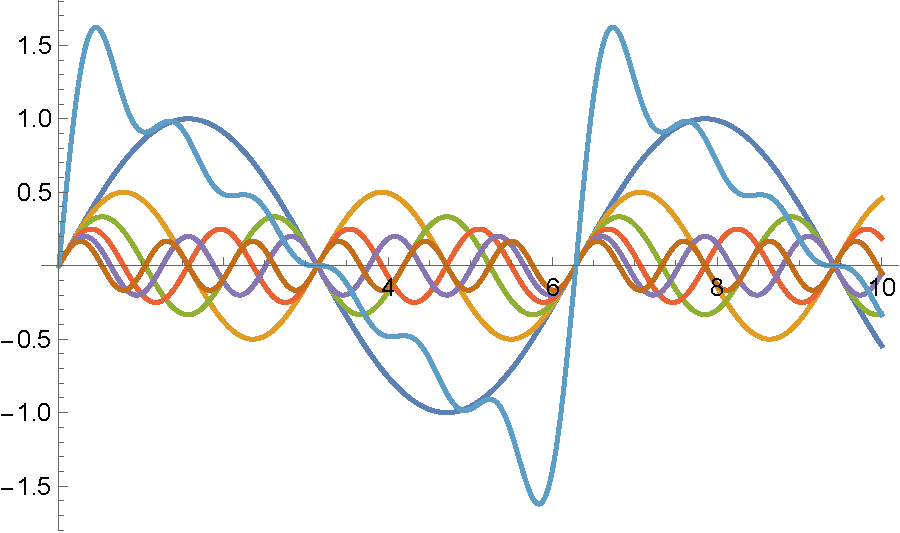
\includegraphics[width = 0.8\textwidth]{Plot1.pdf}
    \end{center}
\end{mathematica}

“呀嘞~看上去蛮有趣的!”地狱妖精兴奋地称赞道。

“是的,这其实是 $\sum_{n=1}^{6} \frac{\sin nx}{n} $ 及其子波图像。”朱鹭子解释道,“反正你们就看着玩就行了。”

“那那……可移动起来吗?”露娜问道。

“动起来啊……”朱鹭子修改了一下当前的代码:

\begin{mathematica}
    Plot[\{\key{\#}, Plus\@\@\key{\#}\}, \{\key{x}, 0, 10\}] \&\@ Table[Sin[\key{n} \UDsymbol{x}] / \key{n}, \{\key{n}, \key{k}\}] \~ Manipulate \~ \{\key{k}, 1, 10\}
    \ShiftEnter
    \begin{center}
        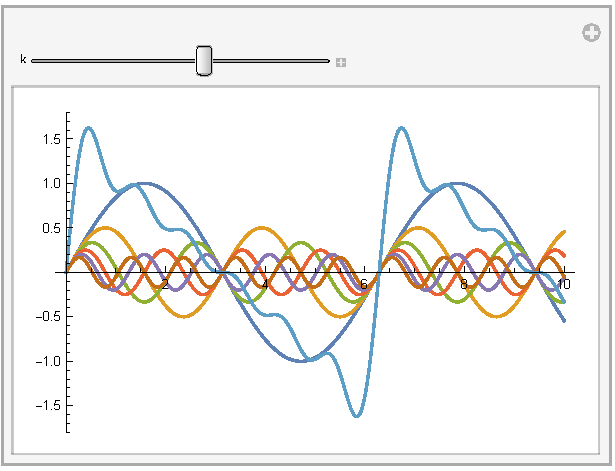
\includegraphics[width = 0.8\textwidth]{Plot3.pdf}\footnote{当然这里是 PDF 交互不了(实现较为麻烦且对 PDF 预览器比较苛刻)。}
    \end{center}
\end{mathematica}

随着 \verb"k" 对应的光标的拖动,函数图像也在进行相应的变化。

“虽然看得出来是边动边计算……不过只用这样少的语句就能写出来确实蛮厉害的。”八云蓝称赞道,“这玩意如果给……(她下意识望了望周围)河童们使用应该会提升不少效率吧?”

“是的,Mathematica 在工程学和物理学上面都有很独特的应用——尤其是其符号推导方面。”朱鹭子用背诵的口吻回答道。“之前演示的各种求导、积分、解符号方程都是例子嘛。”

“哦吼——动起来了!”桑尼睁大眼睛紧紧盯着屏幕,“感觉就像是彩色的蛇在不断爬行一样呢!”

“是的——我们还有更好看的!”朱鹭子说。

\begin{mathematica}
    Plot3D[

    \tab 4(\key{x}\^2 + Sin\@\key{y}\^2)\^2 Exp[1 - \key{x}\^2 - \key{y}\^2] + Sin[\key{x y}],

    \tab \{\key{x}, -3, 3\}, \{\key{y}, -3, 3\},

    \tab MeshFunctions -> \{\key{\#3} \&\}, Mesh -> 20,

    \tab MeshShading -> \{Automatic, Opacity[0.5]\}, PlotPoints -> 200]
    \ShiftEnter
    \begin{center}
        \includegraphics[width = 0.8\textwidth]{Plot4.pdf}
    \end{center}
\end{mathematica}

“3D模型?还是什么?”见到读书妖怪可以肆意地旋转,缩放、移动图形\footnote{在 Mathematica 终端中,旋转可以用鼠标左键拖动、缩放用 \texttt{Ctrl + }鼠标左键,而移动是 \texttt{Alt + }鼠标左键。},八云蓝这么问道。

“差不多吧……实际上这玩意是用很多 \verb"List" 各种嵌套生成的曲面,每一个 \verb"List" 可以代表一个采样点的坐标。将其用 \verb"FullForm" 展开之后,可以看到里面一堆的采样点用 \verb"List" 存储。你说的3D模型本质上也差不多嘛。”朱鹭子解释道。

“除了这个大黄还有什么其他有趣的?”皮斯问道。此时桑尼不知道从哪里拿了一小杯酒交给皮斯,“嘛——”,嘴中未吞咽的食物让她口齿不清,“感觉看不懂,可能露娜更喜欢小玩意吧。”

“喂……怎么又是我?”露娜鼓着栗子嘴吐槽道。

“这里倒是有个很‘炫彩’的东西——和‘复数’相关的。”朱鹭子见状连忙提议道。

\begin{mathematica}
    ComplexPlot[(Sqrt\@\key{z} Log\@\key{z}) / Exp\@\key{z},

    \tab  \{\key{z}, -2 - 2I, 2 + 2I\},

    \tab ColorFunction -> \{

    \tab\tab  Hue[Sqrt\@\key{\#7}, 1 - SawtoothWave[10\key{\#5}]\^20,

            \tab\tab 1 - SawtoothWave[10\key{\#6}]\^20] \&, None

    \tab \},

    \tab RasterSize -> 10000,

    \tab Background -> None]\footnote{事实上这命令运算可能会让电脑轰隆许久,这里建议不要去试(或者将 \texttt{10000} 调小之后去试)。}
    \ShiftEnter
    \begin{center}
        \includegraphics[width = 0.8\textwidth]{Plot5.pdf}
    \end{center}
\end{mathematica}


“哇嘞~这还蛮好看的。”霓虹色的光满慢慢浮在八云蓝的脸上,将她那宝石般的眼睛照得闪闪发亮。

“我天……大姐姐输入了什么代码那么厉害!”露娜叫道。

“现在太晚了,明天找个时间偷偷告诉你。”无名妖怪安慰月之妖精说道,“怎么说?还想看看些什么图?”这最后一句话是对八云蓝说的。

“嘛……分形?”

\begin{mathematica}
    JuliaSetPlot[-0.77 + 0.22 I,

    \tab PlotRange -> \{\{-0.2, 0.8\}, \{-0.8, 0.2\}\},

    \tab PlotLegends -> Automatic,

    \tab ColorFunction -> "{\color{gray}Rainbow}",

    \tab ImageResolution -> 10000,

    \tab Background -> None]
    \ShiftEnter
    \begin{center}
        \includegraphics[width = 0.8\textwidth]{Plot6.pdf}
    \end{center}
\end{mathematica}


“酷!!就好像深邃的漩涡一样恐怖!太棒了!”火炬妖精大叫道,“看这玩意我又感到冷了……这简直就像被深渊巨龙吞噬一般恐怖……”

“我感觉像章鱼怪——呼啦!就那种——会把所有东西都吞掉的那种超级怪物!!”桑尼张牙舞爪地对着露娜和斯塔叫道——“呜哇啊啊啊啊——”妖精们的叫声混杂在一起无法分辨,森林里又充满了快活的空气。

“哈哈,妖精们还真是有活力呢——”霖之助开始打哈欠了,“果然,没有酒水后困意很快就上来了,不过你们带来的梅花酒真的挺厉……看!”

霖之助指着远处,零星灯火正在逐步熄灭——该收摊了。

“嗐——正好我也累了,可惜油豆腐没摸着……要不今天就先这样吧?”八云蓝大度地说。

“也好,”朱鹭子接过台阶,“今晚大家都很尽兴啊……这软件——感觉如何?”最后她还是试探性地问道。

“嗯……怎么说呢……”事实上,两人都已经不是很在意这结果如何了,反正出摊嘛……大家玩得开心就行,至于什么 Mathematica 能不能得到幻想乡数学大师的肯定、这红白软件能不能掀起幻想乡的科技产业革命,其实都不是今晚——或者说今早应该思考的的事情。道理大家都是懂的。

“总之玩得很尽兴就是了,这东西也很厉害——也希望最后这玩意真的能满足河童们那些奇怪的需求吧,这样对大家都好。”最强式神八云蓝,终于作出了明面上的让步,“先收摊吧。”

“嘿!你们比完了吧?!那软件怎么说?!”

听这声音,估摸着还是那地中海河童吧——不错,果然是他。

“怎么样怎么样?”他小跑过来问道,在身后激起一片雪。

“差不多比完了,结果大概就是——”无名妖怪望了下策士,“双赢吧!”她难得用豪爽的声音说道。

“哈!双赢!赢麻啦!”八云蓝笑道。

“所以……这边介意留下联系方式吗,后续河城大人可能会跟您联系下……”年老的河童露出官场笑说道。

“行啦行啦……这边没啥联系方式,你有什么问题就找霖之助吧……从村落大南门沿着兽道一直走,走到第一个岔路口那就写着牌子,之后按告示牌走就行。哦哦不过别把今晚这事大肆宣传。”

“中嘞——为了防止被那资本家听到也确实要偷偷摸摸来,那多谢妖怪小姐了,这边先告辞了。”河童边后退边说,不一会儿就消失得没影了。

不愧是河童速度啊,朱鹭子感叹道。妖怪之山——幻想乡的未来可能还真就托在这软件上了呢。她麻利地关掉电脑,卸下电源,“你们来帮忙吧!”她对远处正要偷偷溜走的妖精们说道。

“啊嘞?啊——好吧好吧……”即使是抱怨也是桑尼第一个带头,虽说如此,她们四个依然走向了霖之助的摊。“一起来吧……”三——四妖精在桑尼一声令下,开始跌跌撞撞的收拾起来。

“诶诶诶额啊啊啊——别碰坏我的电脑啊啊啊啊啊——”

黑夜中,长着翅膀的壮实身影隐于树后。“嘿嘿,还好这玩意小没被搜出来……这下明天总算能够超越文那个家伙了!”黑影窃笑道。

完全没有注意到从身后靠近的九尾妖兽。

\begin{center}
    \section{下半夜}
\end{center}


\begin{tcolorbox}[boxrule=0.5pt, fontupper = \itshapeCJK]
    大家好,这里是本文的作者小飞舞。说来惭愧,本来是要写一篇 Mathematica 的介绍的,结果一时兴起写成了东方的形状,说着说着反倒变成了 Wolfram 语言的介绍了,而且关于副标题中的“一切都是表达式”也没有怎么提及……这里就权当弥补一下,将在文中因为剧情原因不方便说明的内容在此一一说道说道。
\end{tcolorbox}

\subsection{Mathematica 到底有什么用}

作为新生,大家估计会对数学、物理这些学科思维的转变感到陌生,尤其是在面对近乎无理取闹的积分、常微分方程、解析几何这些坏东西,大家可能需要一种方法去对付他们——不是答案,也不是手算,而是通过计算机解决问题。

这是我当时用 Mathematica 的初衷,作为狂拽炫酷吊炸天的最强符号运算系统之一,拿来推作业题的积分、微分方程、级数都完全不在话下。实属新生解决应急数学之痛的必备良药口牙。当然,这玩意也可以用来编程——Wolfram 语言是函数式编程语言,可能写起来会比较“过程性”,用在数据处理和数学符号计算再好不过——写 \verb"For" 循环?那还是算了吧……

正如 Mathematica 强调的那样,Mathematica 可以做很多事情,也可以帮助你学到很多——尤其是那极其有用的帮助文档\footnote{请不要通过看帮助文档的数学名词而称为名词党哦(笑)。}和大量的在线学习课程\footnote{这些课程可以在 \link{https://www.wolfram.com} 上找到。},对新入学的大一新生们大有裨益。

各位看官老爷们也可以看看这里:\link{https://www.zhihu.com/question/27834147} 来感受下 Mathematica(Wolfram) 语言到底有多么神奇。

\subsection{如何部署 Mathematica}

开篇先说明:Mathematica 是要钱的。具体价格可以在 \link{https://www.wolfram.com/mathematica/pricing} 上面找到。

那作为家境贫寒的学生党,如果我们也需要使用那强力的符号运算系统应该怎么办呢?

事实上我们可以这样认为,Mathematica分为两部分,一部分是我们看到的 Mathematica 软件,俗称“前端”。这玩意可以对结果进行调整——比如随手保存图片、拖放图片大小等等,Mathematica 的前端就做得非常的人性化——帮助里的代码甚至都可以直接运行!另一部分我们可以称为是 Mathematica 的 Kernel. 负责所谓的解析输入、计算、返回结果,然后结果由前端来展示。

因此所有的内部计算都需要靠调用 Kernel 来进行,这个 Kernel 我们称为 Wolfram Engine(WE),幸运的是,它是免费的\footnote{当然,免费分各种情形,具体的信息可以参考 \link{https://www.wolfram.com/engine/commercial-options}.}。因此我们可以在 \link{https://www.wolfram.com/engine} 上面下载这 WE 的 Windows, Mac, Linux 版本。

按照网页 / 安装包的提示下载安装Mathematiaca / WE 即可。这期间你需要一个 Wolfram 账号。

\subsection{如何面对 Wolfram 语言}
\setcounter{mma}{0}
\def\mathematicatitlename{Untitled * - Wolfram Mathematica 13.1}



Wolfram 语言与其他很多编程语言都不相同,那就是其非常地“现代化”,就是将大量算法封装在一个个函数中,让大家看不到是如何运作的。我们更像是拼图的组装员,将对应的命令一个个码起来。事实上,Wolfram 语言使得每个人都能够进行尖端的计算——通过其独特的知识网络和丰富的自动化工具。

一眼看上去,Wolfram 语言好像更加“人文”,输入直接就可以得到输出、变量不需要任何声明、空格可以表示乘号、默认超大数支持、会尽可能给出精确的解等等:

\begin{mathematica}
    1 + 1

    f[\texttt{a}]

    3 5

    1000!
    \ShiftEnter
    \xeCJKDeclareCharClass{CJK}{"0030 -> "0039}\CJKfontspec{Iosevka}
    2

    f[a]

    15

    \scriptsize
    402387260077093773543702433923003985719374864210714632543799910429938512398629020592044208486969404800479988610197196058631666872994808558901323829669944590997424504087073759918823627727188732519779505950995276120874975462497043601418278094646496291056393887437886487337119181045825783647849977012476632889835955735432513185323958463075557409114262417474349347553428646576611667797396668820291207379143853719588249808126867838374559731746136085379534524221586593201928090878297308431392844403281231558611036976801357304216168747609675871348312025478589320767169132448426236131412508780208000261683151027341827977704784635868170164365024153691398281264810213092761244896359928705114964975419909342221566832572080821333186116811553615836546984046708975602900950537616475847728421889679646244945160765353408198901385442487984959953319101723355556602139450399736280750137837615307127761926849034352625200015888535147331611702103968175921510907788019393178114194545257223865541461062892187960223838971476088506276862967146674697562911234082439208160153780889893964518263243671616762179168909779911903754031274622289988005195444414282012187361745992642956581746628302955570299024324153181617210465832036786906117260158783520751516284225540265170483304226143974286933061690897968482590125458327168226458066526769958652682272807075781391858178889652208164348344825993266043367660176999612831860788386150279465955131156552036093988180612138558600301435694527224206344631797460594682573103790084024432438465657245014402821885252470935190620929023136493273497565513958720559654228749774011413346962715422845862377387538230483865688976461927383814900140767310446640259899490222221765904339901886018566526485061799702356193897017860040811889729918311021171229845901641921068884387121855646124960798722908519296819372388642614839657382291123125024186649353143970137428531926649875337218940694281434118520158014123344828015051399694290153483077644569099073152433278288269864602789864321139083506217095002597389863554277196742822248757586765752344220207573630569498825087968928162753848863396909959826280956121450994871701244516461260379029309120889086942028510640182154399457156805941872748998094254742173582401063677404595741785160829230135358081840096996372524230560855903700624271243416909004153690105933983835777939410970027753472000000000000000000000000000000000000000000000000000000000000000000000000000000000000000000000000000000000000000000000000000000000000000000000000000000000000000000000000000000000000000000000000000000000000000000000000000000000000000000000000000000000
    \xeCJKDeclareCharClass{Default}{"0030 -> "0039}
\end{mathematica}


这无疑是对新手极端友好的。当然,也有看起来比较烦躁的——比如所有函数都要首字母大写,用方括号来传参等等,看上去都那么离奇,以及那弥漫在整套代码里的语法糖——的确,Wolfram 语言的语法看起来很怪,但也并不是诚心让别人难受。一般来讲,我们在 Wolfram 遇到的很多东西都是“表达式”,我们暂且认为表达式与表达式之间可以用逗号等隔开——比如:


\begin{mathematica}
    \{\UDsymbol{a}, \UDsymbol{b}, \UDsymbol{c}\};

    Sin\@\UDsymbol{x}
    \ShiftEnter
    \[
        \sin x
        .\]
\end{mathematica}


其中的 \verb"{...}" 中,我们隔开了 \verb"a, b, c" 三个表达式,这仨玩意实际上是列表的参数,整个第一行亦是表达式,用分号与第二个表达式隔开。因此我们可以认为这玩意就是表达式传参到函数的嵌套。至于 \verb"x" 本身,我们可以认为它是符号(Symbols),当然也可以认为是表达式,这点无伤大雅\footnote{事实上,我们一般认为构成表达式的主要是由数字、字符串和符号。}。

有了表达式我们就可以分析表达式的结构了——一般认为,大多数表达式都是由\textbf{表头}(Head)和\textbf{参数}构成——比如说 \verb"Sin@x" 的表头就是 \verb"Sin",至于 \verb"Sin" 本身又是作为什么存在的,其实是 Symbol,因此我们完全可以把函数的名称——表头当成参数传递给函数:



\begin{mathematica}
    ReplaceAll[\{\UDsymbol{a}, \UDsymbol{b}, Sin\@\UDsymbol{c}\}, Sin -> Cos]
    \ShiftEnter
    \{a, b, Cos[c]\}
\end{mathematica}

这样看来,实际上这些乱七八糟的东西都可以当成参数传递进去。你可能会问 \verb"Sin -> Cos" 是怎么传递参数的,问得好!我们可以用 \verb"FullForm" 查看:

\begin{mathematica}
    Sin -> Cos // FullForm
    \ShiftEnter
    Rule[Sin, Cos]
\end{mathematica}

因此,实际上是一个\textbf{匹配规则}:将表达式中所有的 \verb"Sin" 全部变成 \verb"Cos",子表达式也不放过。事实上,由于 \verb"ReplaceAll" 或者说 \verb"/." 只对所有表达式 / 子表达式匹配一次,因此不需要担心递归循环:

\begin{mathematica}
    ReplaceAll[\{\UDsymbol{a}, \UDsymbol{b}, Sin\@\UDsymbol{c}\}, Sin -> Sin]
    \ShiftEnter
    \{a, b, Sin[c]\}
\end{mathematica}

谈到这里,我们就不得不提及列表这个玩意了,列表——之前在文中提过,是一个以 \verb"List" 为表头的表达式——实际上 Wolfram 语言中对列表的操作是重中之重,比如可以选取表达式参数的 \verb"Part":

\begin{mathematica}
    (\UDsymbol{x} + \UDsymbol{y} + \UDsymbol{z}) [[2]]

    Part[\{\UDsymbol{x}, \UDsymbol{y}, \UDsymbol{z}\}, 1]
    \ShiftEnter
    y

    x
\end{mathematica}

我们可以认为 \verb"Part" 对 \verb"FullForm" 形式工作,因此可以对表达式的每一个部分进行细致的改造——又或者是 \verb"Cases": 匹配表达式中的特定模式,然后将匹配结果以列表输出。

\begin{mathematica}
    Cases[\{\UDsymbol{a}, \UDsymbol{y}, \UDsymbol{z}\}, \UDsymbol{a}]
    \ShiftEnter
    \{a\}
\end{mathematica}

看上去好像平平无奇,但实际上我们没有用到 Wolfram 强大的模式匹配功能——这个下划线 \verb"_" 大家可能看着就开始烦躁,这玩意叫做 Blank,可以匹配所有表达式——

\begin{mathematica}
    Cases[\{\UDsymbol{a}, \UDsymbol{y}, \UDsymbol{z}, Cos\@\UDsymbol{z}, \UDsymbol{x}!\}, \_]
    \ShiftEnter
    \{a, y, z, Cos[z], x!\}
\end{mathematica}

当然,要是全匹配了,那也就没什么用了——我们可以给匹配加限定条件,比如说用 \verb"_Head"\footnote{事实上 \texttt{Head} 本身也是一个表头的名字,此处的意思仅仅是可以用此方法来匹配特定表头的表达式。}来匹配特定表头的表达式,或者用在表达式 Blank 前面加标签来表示特殊的模式——

\begin{mathematica}
    Cases[\{\UDsymbol{a}, \UDsymbol{y}, \UDsymbol{z}, Cos\@\UDsymbol{z}, \UDsymbol{x}!\}, \_Cos]

    Cases[\{Cos[Cos], Cos[Sin], Sin[Sin]\}, x\_\@x\_]
    \ShiftEnter
    \{Cos[z]\}

    \{Cos[Cos], Sin[Sin]\}
\end{mathematica}


接下来我们不妨将目光看向函数定义的方面——

\begin{mathematica}
    f[\key{x\_}] := \key{x};
    \ShiftEnter
\end{mathematica}

我们用到了用 \verb"x" 标记的任意表达式,在 \verb":=" 后面可以用 \verb"x" 来指代该表达式,同时呢,我们还用上了 \verb":=",这个称为延迟赋值,我们可以这样理解:由于 Mathematica 函数的定义是匹配型的,我定义了之后 \verb"f" 是什么?其实仍然是个Symbol,只不过当 \verb"f[表达式]" 这个模式出现时,会被我匹配到,从而替换成 \verb":=" 右边那个,而实际上 \verb":=" 并不是真正意义上的赋值,而是等到函数被调用的时候再重新计算\footnote{你会发现我们的输入是用的 \texttt{In[\textit{n}]:=} 而输出是 \texttt{Out[\textit{n}]=},那以后你每次调用输入结果(可以用 \texttt{\%})时其都会重新计算。}——因为如果 \verb"=" 右边的值可以提前被确定的话,那就是正儿八经的赋值了。\footnote{与其对应的有延迟匹配规则 \texttt{:>},其在每一次被调用匹配时都会重新计算右边的值。}

\begin{mathematica}
    f[\key{x\_}] := RandomReal[];

    g[\key{x\_}] = RandomReal[];

    \{f[3], f[3], g[3], g[3]\}
    \ShiftEnter
    \{0.332218, 0.461628, 0.037835, 0.037835\}
\end{mathematica}

此时 \verb"g[_]"\footnote{要注意到 Blank 也是表达式,同样会被匹配。} 的值已经被完全确定,因此我们定义函数的时候会采用 \verb":=".

但定义函数是相当麻烦的——如果要想其他语言那样的话,我需要用各种标签标记表达式,然后凑成一块——但有时候我仅仅用个临时函数而已啊?!因此我们需要用匿名函数——你可能会对这些 \verb"#, &, @" 产生抵触,但这其实也是语法的一部分。

这是一个简单的 $\lambda $ 表达式:

\begin{mathematica}
    \key{\#}\&

    \key{\#}\&[3]
    \ShiftEnter
    \#1\&

    3
\end{mathematica}

其中 \verb"#" 是 \verb"Slot",即“槽”,我们可以认为 \verb"#n" 代表第 \verb"n" 个参数,至于 \verb"&"……其实是函数的表征,我们可以将其认为是 \verb" // Function"\footnote{此处的运算顺序可能有些不同,这里仅仅是便于理解。},这样我们就得到了一个类似 \verb"Function[#]" 的东西了,我们会认为这是个函数(实际上它的表头的确是函数:\verb"Function[Slot[1]]"),那么应该怎么用呢?

没错,我们可以把它当成表头给其传参——

\begin{mathematica}
    \key{\#}\^2\&\@\UDsymbol{x}
    \ShiftEnter
    x\^{}2
\end{mathematica}


然后就有了这看起来非常哈人的三个连在一起的特殊字符。当然这样不好一次性传多个参数,我们也可以用(其实本就更应该用)方括号传参——

\begin{mathematica}
    Cos\@\key{\#2}\@\key{\#3}\key{\#}\&[\UDsymbol{x}, Sin, \UDsymbol{t}]\footnote{这最后面的 {\ttfamily\#3\#} 可能会感觉很怪,但实际上是 {\ttfamily\#3} 与 {\ttfamily\#} 的乘积。}
    \ShiftEnter
    x Cos[Sin[t]]
\end{mathematica}

有了这玩意,我们就可以通过后缀运算和匿名函数来实现可读性更强的代码:

\begin{mathematica}
    Sin\@\UDsymbol{x} // \{Table[Series[\key{\#}, \{\key{x}, 0, 2\key{n}\}], \{\key{n}, 4\}], \key{\#}\} \& // Normal // Plot[\key{\#}, \{\key{x}, -Pi, Pi\}] \&
    \ShiftEnter
    \begin{center}
        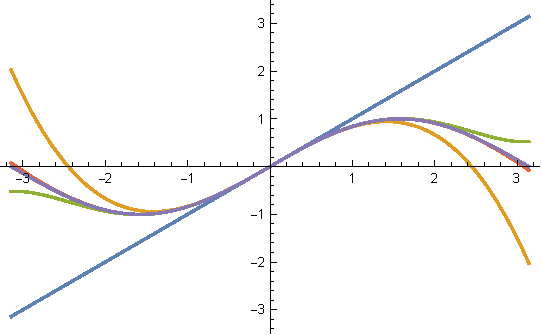
\includegraphics[width = 0.8\textwidth]{Plot7.pdf}
    \end{center}
\end{mathematica}

代码的可读性当然是相当重要的——除非你在参加什么比赛要尽可能写短的代码,如果我们将表头从前到后一直读下来,就能明白代码的大体意思,那自然是再好不过的。

\subsection{参考资料}

事实上,我觉得 Mathematica 的 UI 比 MATLAB 和 Maple 都要好,这同样体现在其帮助 (Help) 的 UI 上面。

\begin{tcolorbox}[
        enhanced,
        clip upper = true,
        left = -3pt,
        top = -3pt,
        right = -3pt,
        bottom = -3pt,
        colframe = lightgray!40!white,
        title = {\
                \begin{tikzpicture}
                    \filldraw[macred] (0, 0) circle (0.3em);
                    \filldraw[macyellow!80!white] (0.5, 0) circle (0.3em);
                    \filldraw[macgreen] (1, 0) circle (0.3em);
                \end{tikzpicture}%
                \hfill{\footnotesize\sffamily https://reference.wolfram.com/language/index.html.zh}\hfill%
                \phantom{
                    \begin{tikzpicture}
                        \filldraw[macred] (0, 0) circle (0.3em);
                        \filldraw[macyellow!80!white] (0.5, 0) circle (0.3em);
                        \filldraw[macgreen] (1, 0) circle (0.3em);
                    \end{tikzpicture}
                }
            }, coltitle = black, colbacklower = red!20, height = 0.6\paperheight-20pt, breakable
    ]
    \makebox[\width][c]{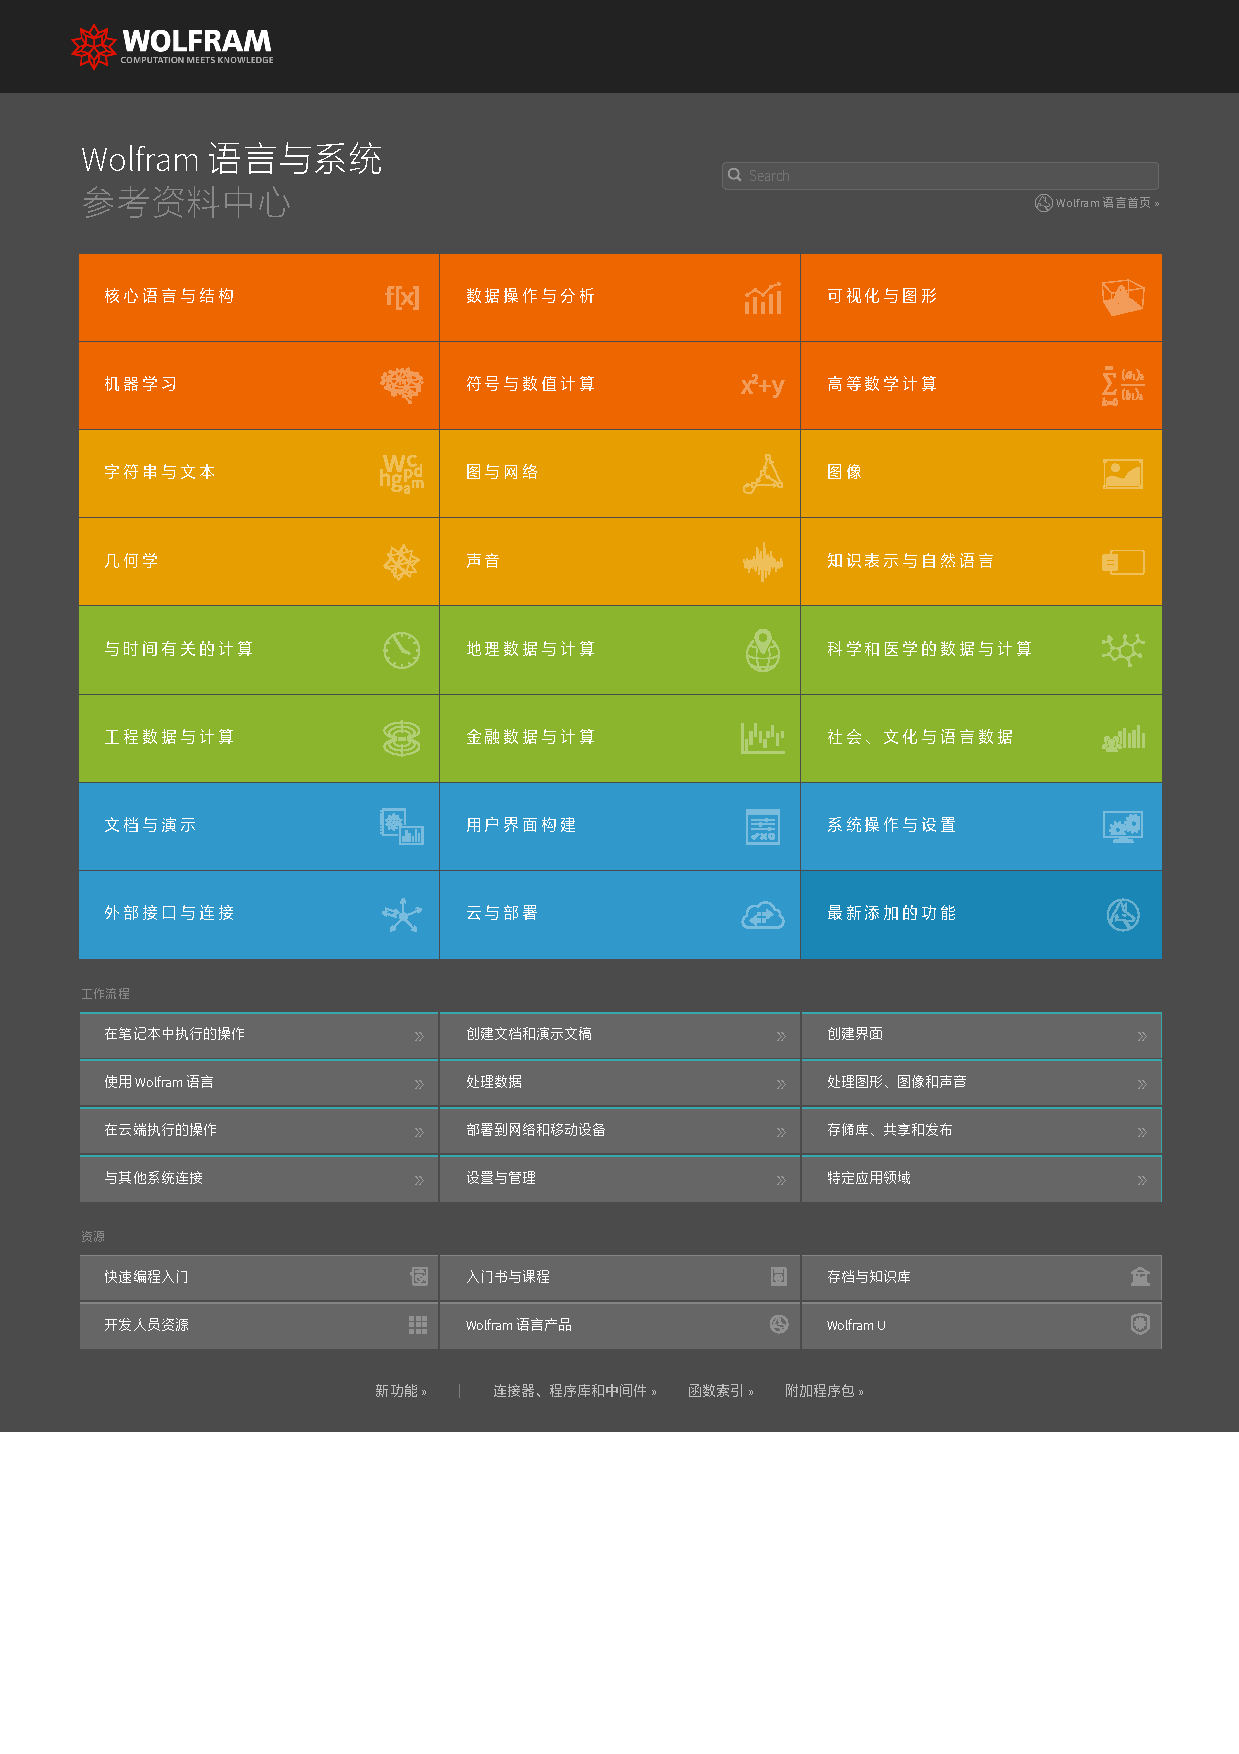
\includegraphics[width = \linewidth]{Wolframdoc.pdf}}
\end{tcolorbox}

Mathematica 的帮助已经相当面面俱到——对入门的新手实在是没有什么比其更好了。如果在 Mathematica 终端中打开帮助
(\verb"F1"),则帮助中的示例代码可以实时修改后运行,对那些乱七八糟的内置函数,在那里乱扯一通工作原理还不如看例子学习得快。

当然,如果你不满足需要撞到问题了再去浩如烟海的帮助中寻迹,那可以在此查看快速的编程入门 \link{https://www.wolfram.com/language/fast-introduction-for-programmers/zh/},更深入的可以了解 \link{https://www.wolfram.com/language/elementary-introduction/2nd-ed/},又称 \textcite[AN ELEMENTARY INTRODUCTION TO THE Wolfram Language]{wolfram2017},这玩意有实体书(当然也有 PDF,这 PDF 据称是用 Mathematica 排版的)。

另外、如果在实际工作用遇到了什么问题,也可以在 \href{https://mathematica.stackexchange.com/}{Mathematica Stack Exchange} 或者是 \href{https://community.wolfram.com/}{Wolfram Community} 上提问。

\subsection{作业}

哈!这里当然不是什么正经作业——不过我觉得还算是一个蛮有趣的简单练习:

\itshapeCJK\begin{enumerate}%
    \item 大家可能使用 \LaTeX 写笔记,其中可能需要进行简单的函数绘图——我们清楚这当然可以用 Mathematica 完成,但是小飞舞同学有时候更喜欢用 PGFPlots 宏包来绘图:
\begin{lstlisting}
    \begin{tikzpicture}
        \pgfplotsset{width = 12cm, height = 5.5cm}
        \begin{styleedaxis}[
                axis x line                           = middle,
                axis y line                           = middle,
                every inner x axis line/.append style = {->},
                every inner y axis line/.append style = {->},
                title                                 = $\exp x$,
                ymax                                  = 26,
                xlabel                                = $x$,
                ylabel                                = $y$,
            ]
            \addplot[
                domain = -3.5: 3.5,
                thick
            ]{e^x};
        \end{styleedaxis}
    \end{tikzpicture}
\end{lstlisting}

          \begin{center}
              \begin{tikzpicture}
                  \pgfplotsset{width=12cm,height=5.5cm}
                  \newcommand{\function}{e^x}
                  \begin{axis}[
                          axis x line=middle,
                          axis y line=middle,
                          every inner x axis line/.append style={->},
                          every inner y axis line/.append style={->},
                          title={$\exp x$},
                          ymajorgrids=false,
                          xmajorgrids=false,
                          grid style=dashed,
                          samples=1000,
                          ymax = 26,
                          xlabel = $x$,
                          ylabel = $y$,
                      ]
                      \addplot[
                          domain=-3.5: 3.5,
                          thick
                      ]
                      {\function};
                  \end{axis}
              \end{tikzpicture}
          \end{center}
          这宏包调用的是 PGFMath,这玩意绘图速度实在是太太太慢了!而且重点是不支持一些特殊函数。比如说我要画第一类贝塞尔函数\footnote{实际上可以调用 GNUPlot 绘图,这玩意支持 Bessel 函数的绘制。} $\operatorname{J}_0(z) =  \sum_{n=0}^{\infty} \frac{(-1)^n}{4^n(n!)^2}z^{2n}$ 就相当麻烦。事实上这宏包可以调用离散点进行绘图,具体可参考 \textcite[PGFPlots 文档]{feuersanger2011manual}——总之就是用
\begin{lstlisting}
        x1  y1  
        x2  y2  
        x3  y3  
        x4  y4  
        ......
\end{lstlisting}
          进行离散点输入。

          那你现在有着最强符号运算系统之一,请你写个小程序让 Mathematica 输出这种形式的坐标,然后给 PGFPlots 绘图。

          顺便试试隐函数绘图和参数方程的绘图(笑)。
    \item 在使用 Mathematica 的过程中,有时候会见到两个 \texttt{\#} 连在一起的情况,如\texttt{\#\#\textit{n}},这被称为 SlotSequence,一般在 $\lambda$ 表达式中使用,表示从第 \texttt{\textit{n}} 个开始直到结束的参数序列:
          \begin{mathematica}
              \comment{(*将一个列表复制一份跟在后面的函数*)}

              f[\key{list\_}] := \{\key{\#\#}, \key{\#\#}\} \&\@\@ \key{list};

              f[\{1, 2, 4\}]

              \comment{(*从第二个参数开始*)}

              g[\key{list\_}] := \{\key{\#\#2}, \key{\#\#2}\} \&\@\@ \key{list};

              g[\{1, 2, 4\}]
              \ShiftEnter
              \{1, 2, 4, 1, 2, 4\}

              \{2, 4, 2, 4\}
          \end{mathematica}

          嘛……看上去也是平平无奇,那……请解释下面俩代码的差异:

          \begin{mathematica}
              f[\key{\#\#2\#1}] \& \@\@ \{1, 2, 3, 4, 5, 6, 7, 8, 9, 10\}

              f[\key{\#\#2}] \& \@\@ \{1, 2, 3, 4, 5, 6, 7, 8, 9, 10\}
              \ShiftEnter
              3628800

              f[2, 3, 4, 5, 6, 7, 8, 9, 10]
          \end{mathematica}

          即乘上一个 \texttt{\#1} 到底发生了什么?
\end{enumerate}

\upshape

\vfill
\begin{center}
    
\includegraphics{wolframLanguage.pdf}
\end{center}
\vfill\mbox{}
\clearpage